\documentclass[../main.tex]{subfiles}

\begin{document}
\chapter*{Notacja}

\begin{tabularx}{\textwidth}{cl}
  $\chi^{+}(a)$ 
  & funkcja pomocnicza równa $1$ gdy $a>0$, 0 w przeciwnym przypadku \\
  
  $\mathbb{R}^{\text{surf}}$
  & reflektancja powierzchniowa \\
  
  $\mathbb{R}^{\text{vol}}$
  & reflektancja ciała \\
  
  $n$
  & współczynnik załamania \\
  
  $Q$
  & energia \\
  
  $\Phi$ 
  & strumień promieniowania \\
  
  $B$
  & radiosity \\
  
  $E$
  & irradiancja \\
  
  $\omega_o$
  & kierunek w którym światło kontynuuje swoją drogę \\
  
  $\omega_i$
  & kierunek z którego światło przybywa \\
  
  $L$
  & radiancja \\
  
  $L_i$
  & radiancja wychodząca \\
  
  $L_o$
  & radiancja przychodząca \\
  
  $f_r$
  & BRDF \\
  
  $\rho$ 
  & bihemispherical reflectance, albedo \\
  
  $D$
  & funkcja rozkładu normalnych NDF, w rozdziale \ref{Chapter:LTC} oznacza pewien rozkład \\
  
  $F$
  & funkcja Fresnela \\
  
  $G$ 
  & funkcja geometryczna \\  
\end{tabularx}

\begin{figure}[h]
    \centering
    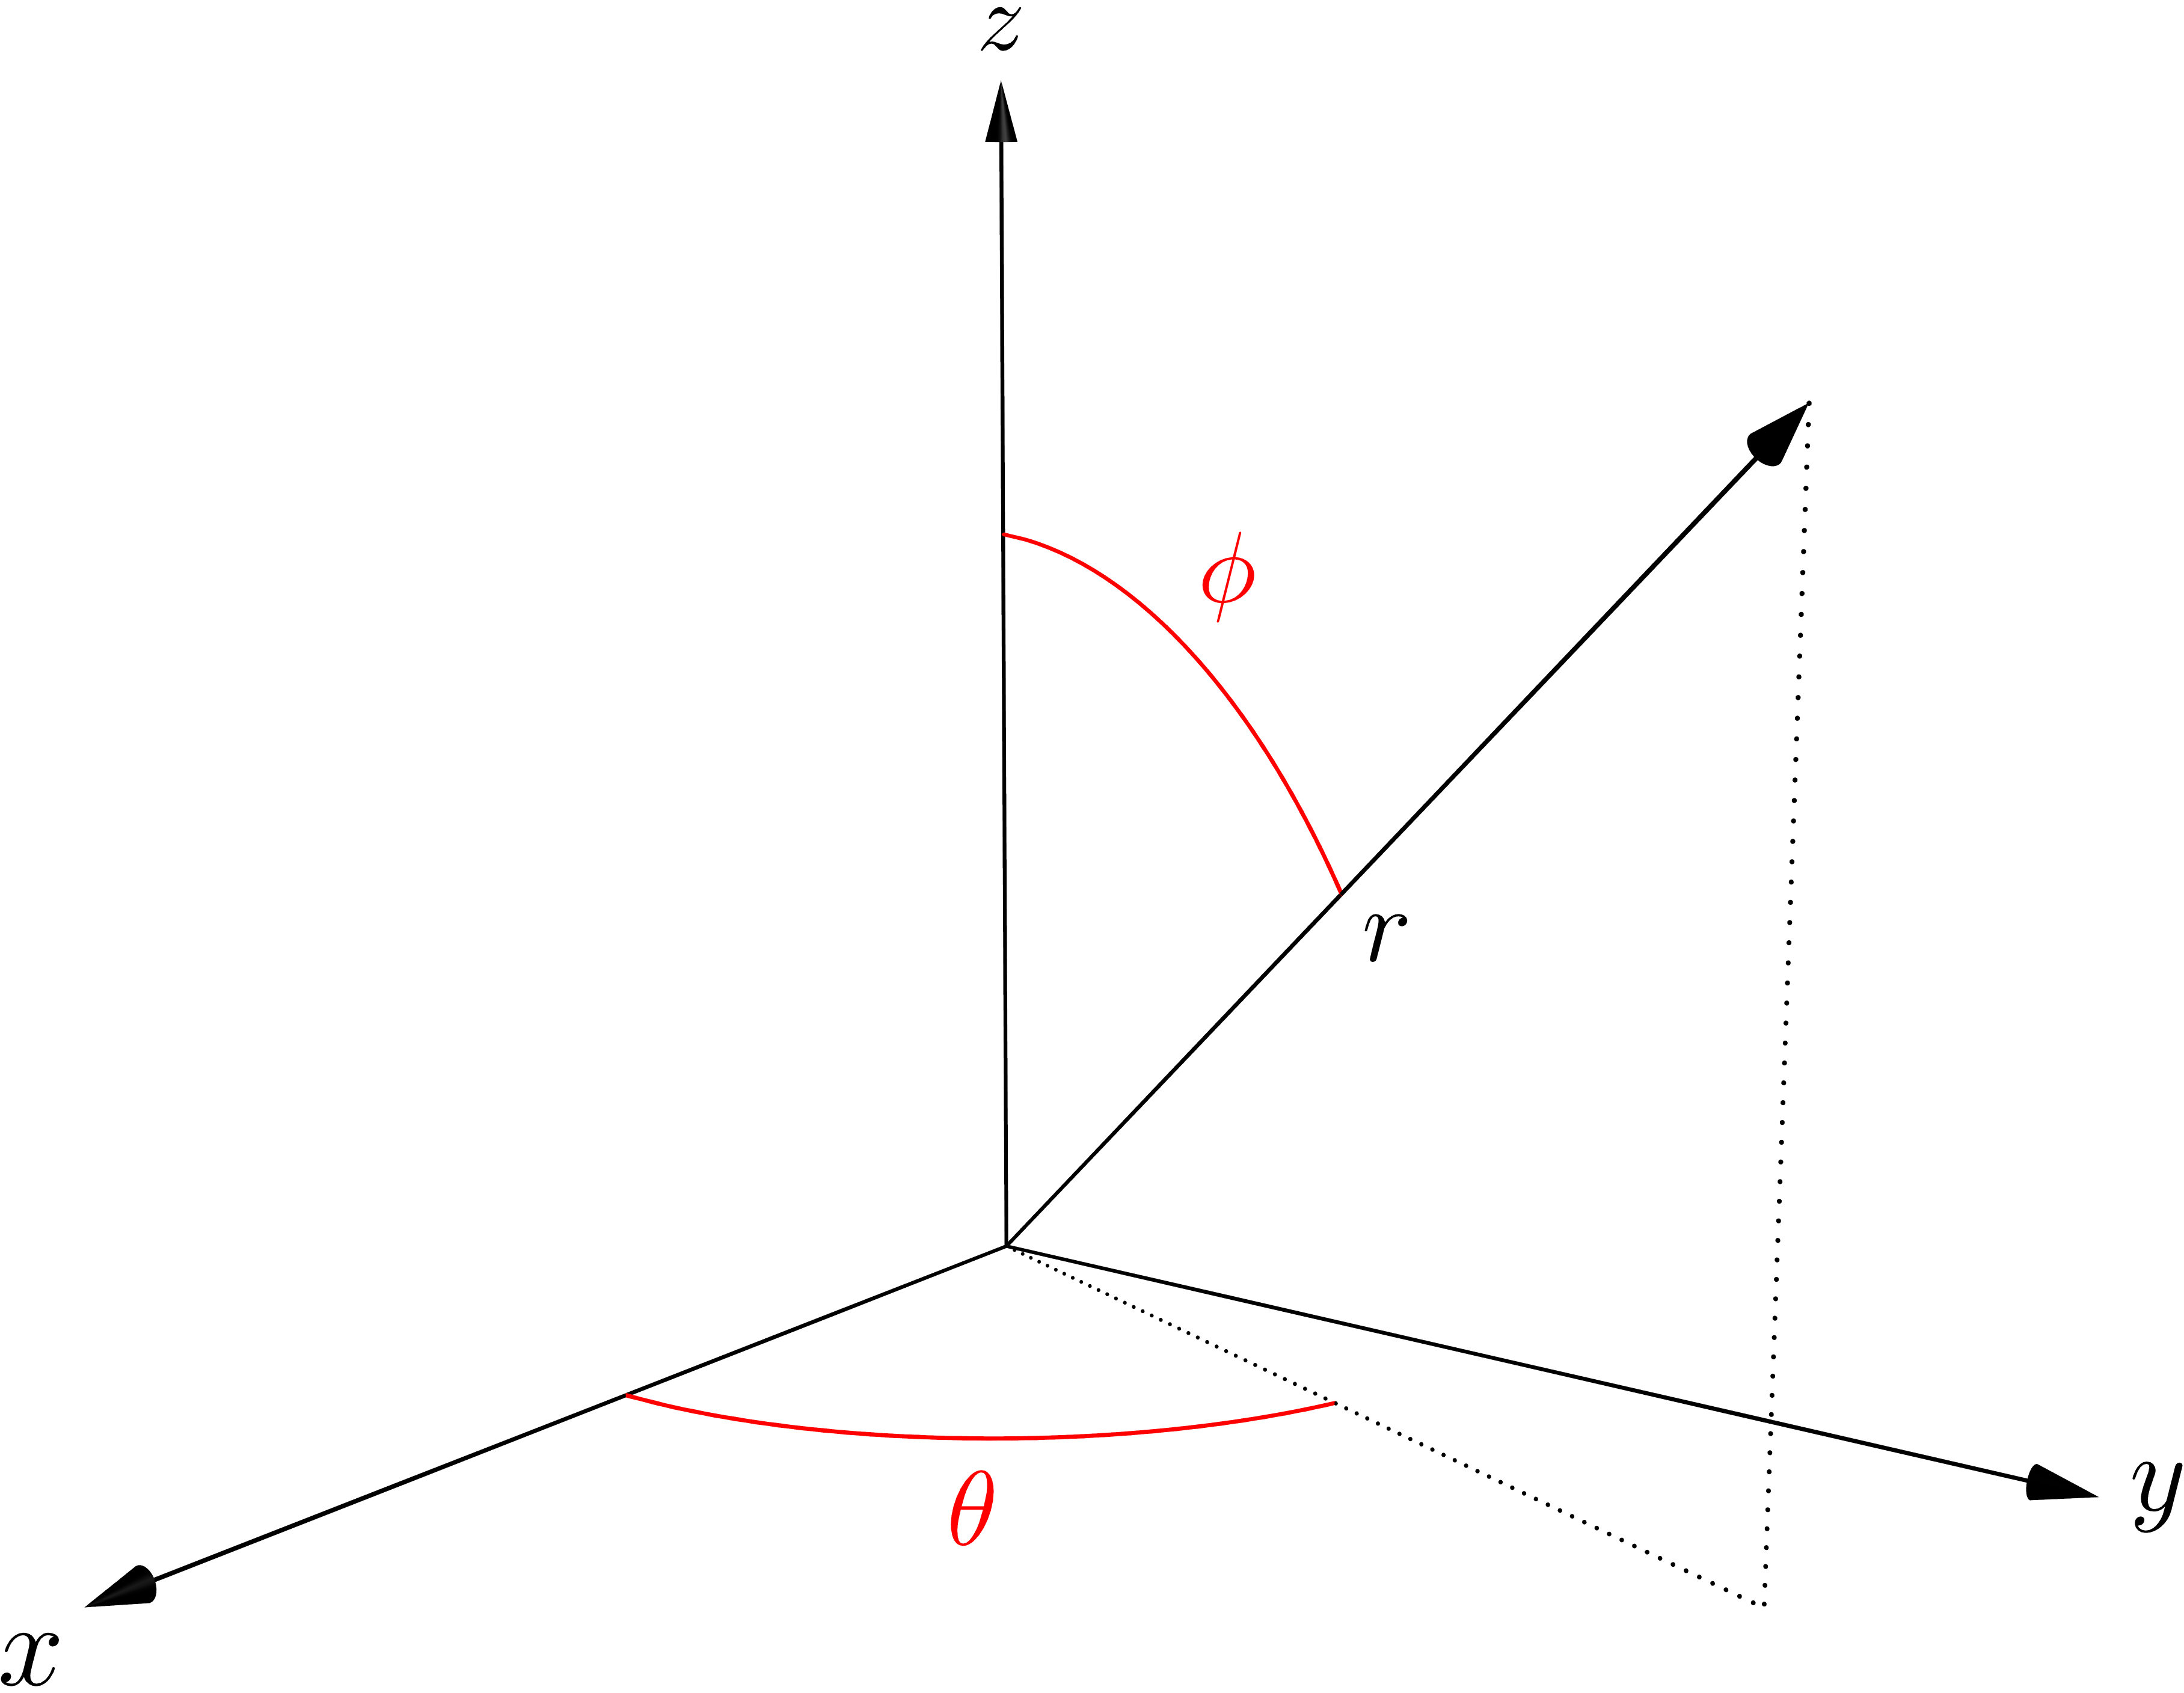
\includegraphics{notation/angles}
    \caption{Układ współrzędnych i kąty sferyczne stosowane w pracy. Opracowanie własne.}
    \label{fig:NotationAngles}
\end{figure}

\end{document}
